\documentclass{svproc}
\usepackage{graphicx}  %%% for including graphics
\usepackage{url}
\tolerance=1
\emergencystretch=\maxdimen
\hyphenpenalty=10000
\usepackage{caption}
\usepackage{float}
\usepackage[ruled,vlined]{algorithm2e}
\usepackage{algorithmic}
\usepackage{array}
\usepackage{tabularx}
\usepackage{subcaption}
\usepackage{makecell}
\def\UrlFont{\rmfamily}
\captionsetup{compatibility=false}


\begin{document}
\mainmatter
\title{Using image difference as a heuristic for solving 8-puzzle problem}
\subtitle{CS7IS2 Project (2019/2020)}
\author{Kulkarni Shravani Deepak, Kapoor Shuchita, Asolkar Jayprakash, Chauhan Paritosh}

\institute{
\email{kulkarsh@tcd.ie, kapoorsh@tcd.ie, asolkarj@tcd.ie, chauhapa@tcd.ie}\linebreak School of Computer Science and Statistics, Trinity College Dublin}

\authorrunning{Kulkarni Shravani Deepak et al.}

\maketitle

\vspace{0cm}
\begin{abstract}
The 8-puzzle problem remains a well-researched game in the AI domain and is used to test the efficiency of various search algorithms. In this analysis, we apply the A* algorithm with Hausdorff distance as heuristic function on the 8-puzzle grid that involves images of state spaces instead of number array. Additionally, the research obtains interesting results by comparing the performance of the chosen method with other search strategies such as BFS, DFS and A* with Gaschnig’s Max Swap heuristic. The research showed that the chosen method gave the least number of expanded nodes even though it took more time than the baseline strategies.
\keywords{artificial intelligence, 8 puzzle, BFS, DFS, A*, Hausdorff distance, Gaschnig’s Max Swap}
\end{abstract}
%

 

\section{Introduction}
\noindent The Artificial Intelligence domain has had many single-agent search algorithms. To check their effectiveness, numerous gaming problems have been developed. Among these games is the N-puzzle problem, which is also included in the list of classic difficulty issues. This puzzle is made up of N square tiles numbered from 1 to N. It is represented in a search graph or tree, where the nodes depict the position of the square tiles in the grid. The goal of this problem is to rearrange the numbers in ascending order on the MxM board. \\

\noindent  This paper focusses on the 8-puzzle problem, which was chosen because it has a smaller state space than the larger N-puzzle problem and the algorithms can be analyzed extensively. We have used three algorithms (BFS, DFS, A*) to find the solution for this puzzle. Such solutions are often measured by analyzing their measurement criteria, such as the cost of the path, the time taken and the nodes expanded to find the solution. In the A* algorithm, we have used two heuristic measurements - Gaschnig’s Max Swap and Hausdorff distance. The Hausdorff distance is a novel technique that has not been used in the previous literature to solve the N-puzzle problem. In this technique, the images of the board's current state and the goal state are compared to indicate how far the current state is from the goal state. That is, the difference between the images is used as a heuristic for the A* algorithm. We have evaluated this technique using BFS, DFS and A* with Gaschnig’s Max Swap heuristic as a baseline.  \\

\noindent The paper is structured as follows: section 2 discusses prior literature outlining the algorithms which will be used in this paper,  section 3 defines the 8-puzzle problem in detail and describes the algorithms used, section 4 shows the results and comparisons of these algorithms, section 5 concludes this paper.

\section{Related Work}
\noindent According to the Pearl, et. Al. {\cite{pea}}, the environment that provides a platform for the search is known as Problem Space. Each of these problem spaces consist a set of states and operators. For instance, in terms of 8 puzzle, states can be defined as the different possible arrangement from the initial configuration of the numbers while operators are the possible directions, i.e. Left, Right, Up or Down. The problem instance can be defined as the problem space that consists of initial state and the goal state with a solution. The solution in this case is defined as the set of operators that changes the state from initial to the goal state. To provide the same perspective in terms of visualization, the problem space is considered as a graph (generally a tree) where each state is defined by the node and each operator is illustrated as an edge between the nodes. In searching problem space, there are many methods than can be applied to get to the goal state. We begin with the BruteForce search methods which includes Breadth-First Search, Depth-First Search. This will be followed by a deeper study on the Heuristic Search that includes the A* algorithm.\\

\noindent BFS is an uninformed search algorithm that generates its state space by registering all the nodes that have been traversed in the search tree. For instance, the initial state in the 8-Puzzle problem is considered as the root node and offspring nodes are generated in such a way that the neighbouring nodes represent a single move or state change from the parent. This strategy employs the Breadth-First traversal approach, where the adjacent neighbours are traversed to find the optimum state. The lower levels are generated and traversed only if the required state is not reached on the current level of the tree. This way BFS always provides an optimized solution for a problem. BFS uses FIFO (First in First out) principle for performing search. The time complexity in finding the optimum state is directly proportional to the size of the search space, i.e O($b^{d}$). As all states need to be stored to generate the next level, higher space complexity is the disadvantage of BFS algorithm.\cite{tab}\\

\noindent In comparison to BFS, the idea of DFS is to keep expanding the state till it reaches the optimal solution or backtracking to the next nearest possible state. The algorithm employs LIFO (Last in First Out) approach in order to search the desired state in the search space. The time complexity does not change and remains same as in BFS O($b^{d}$). DFS has better space complexity, where only current search path is being saved (O(d)). This algorithm lacks the ability to provide an optimal solution in the given time and hence sometimes must be provided with an explicit cut-off depth.  The tree search version of DFS also lacks completeness due to possible infinite loops\cite{rus}.\\

\noindent A* is a form of informed search algorithm. The algorithm is made aware about the state space in the notion of heuristic function. The amount of match between a node and the goal state is quantified using the heuristic function which is the difference between the current state from the goal state. The higher value of this function signifies lesser relevancy of that state in reaching towards the goal. The algorithm uses the Breadth-First Search horizontal expansion technique but limits these expansions only to those nodes which have the smaller heuristic function value and also considers the path cost to the goal. A* performs better in terms of space complexity when compared to DFS  and  improves on the time complexity  when compared to BFS. The only disadvantage of using this algorithm is the computational overhead that is required for calculating the heuristic value along with the path cost of each node that is considered.\\

\noindent To solve the 8-puzzle problem, we have chosen to implement Breadth-First Search, Depth-First Search, A* algorithms. With these selected algorithms we can compare both uninformed and informed search techniques in terms of completeness, space-time complexity, and optimality. Although the exhaustive traversal method of both breadth-first and depth-first searches do not promise optimality, they can act as a baseline for comparison with other algorithms in terms of improvements. Whereas the A* algorithm makes use of heuristics to make informed search traversal and provides an optimal solution. With an evaluation function that combines both the cost to reach the current state and estimated cost to reach the goal from the current state, the A* algorithm is both optimal and complete\cite{rus}. Our intention to select the above algorithms is to evaluate the performance of these basic search algorithms on a real-world AI problem such as the 8-puzzle and compare various aspects of the algorithms.\\

\noindent For the study of A* algorithm we have compared Gaschnig’s Max Swap\cite{swa} and Hausdorff distance heuristic evaluation functions. Huang-Chia Shih et al. (2019) have used the Hausdorff distance to solve the problem of Jigsaw Puzzle for reconstruction without template image\cite{shi}. The same can be applied to the 8 puzzle problem involving images of the state space. Gaschnig's evaluation function calculates number of tiles to be shifted to attain goal state if any tile could be swapped with empty tile.

\section{Problem Definition and Algorithm}
 The n-puzzle problem is a classic AI problem which contains n numbered tiles and one blank tile. The tiles are numbered as 1, 2, 3 .. n. The numbered tiles can be moved in the place of empty tile. To achieve the goal state of the puzzle, the grid should be arranged in such a way that the empty tile is at the first position and all the numbered tiles are arranged in numerical order. The aim of the n-puzzle problem is to reach the goal state with the least cost. For instance, an eight-puzzle problem consists of 8 numbered tiles - 1, 2, 3, 4, 5, 6, 7, 8. The goal state of the 8-puzzle problem is shown in Figure~\ref{fig:1a}. \\

\begin{figure}
	\centering
	\begin{subfigure}[b]{0.25\textwidth}
		\centering
		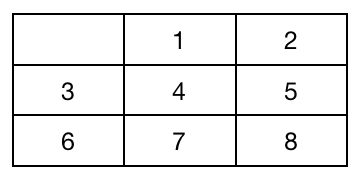
\includegraphics[width=3cm,height=3cm,keepaspectratio]{GoalState.png}
		\caption{Goal State}
		\label{fig:1a}		
	\end{subfigure}
	\begin{subfigure}[b]{0.6\textwidth}
		\centering
		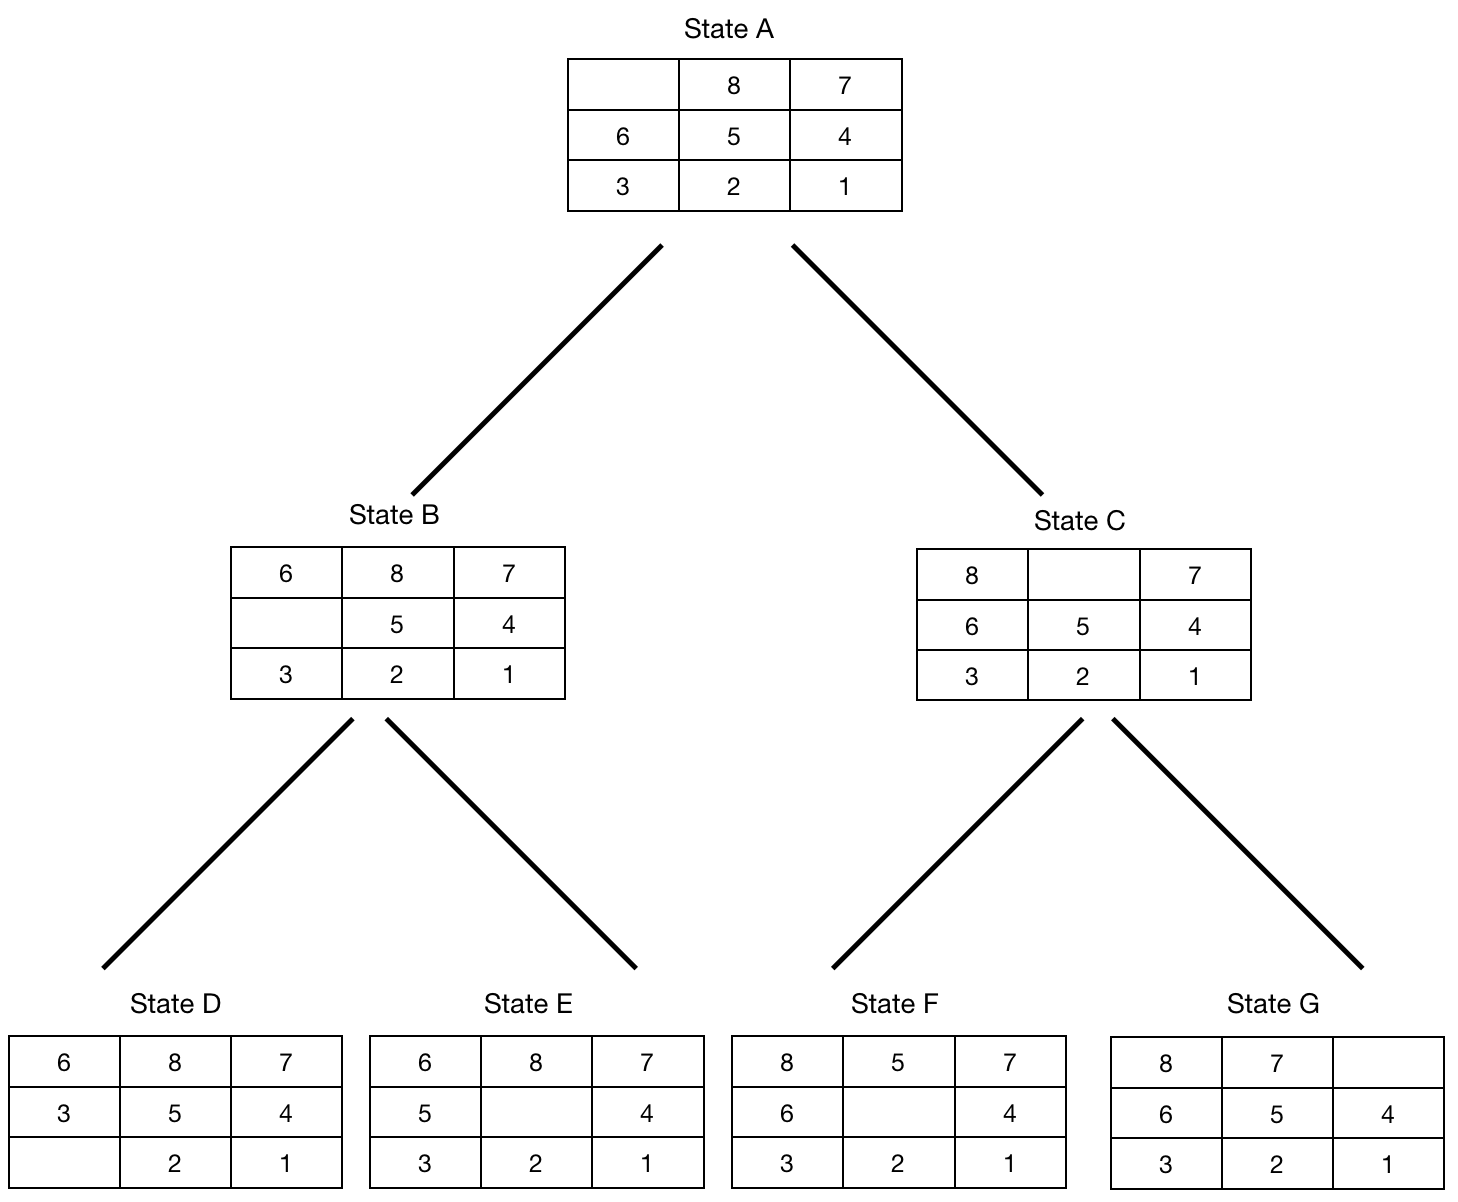
\includegraphics[width=8cm,height=8cm,keepaspectratio]{ExampleState.png}
		\caption{State space of 8-puzzle problem}
		\label{fig:1b}
	\end{subfigure}
	\caption{8 Puzzle Goal State and State Space}
	\label{fig:1}
\end{figure}

\noindent The cost to achieve the goal can be measured in terms of the number of movements done. At any given intermediate state, there can be at least two and at most four possible movements of the blank tile. Although reaching a goal in such puzzles is easy, but finding the shortest path with the lowest cost is difficult. The Figure~\ref{fig:1b} shows an example of a solution for an 8-puzzle problem from the given start state. The state-space of the 8-puzzle problem is such that if the goal state can be achieved in a certain number of steps, then all movements towards the solution are considered good moves and all the movements that are farther from the solution are considered bad moves. The aim is to find the good moves which lead to minimum cost. \\

\noindent 8-puzzle problem is a search problem which can be solved by various searching algorithms like BFS and DFS. In these, the problems are represented as search graphs or trees. The nodes of the graph/tree denote the states where the goal state is also present as one of the nodes. A part of the tree for the 8-puzzle problem is shown in the Figure~\ref{fig:1b}. The searching can be done by expanding to a depth (child nodes) or exploring the breadth (sibling nodes). \\

\noindent For the implementation of BFS, DFS and A*, we referred to an existing implementation\footnote{Github Repository: https://github.com/speix/8-puzzle-solver}, which used Python. The model of a state was built with parameters like state, parent, cost, depth to maintain information about each state. For the 8-puzzle problem, a state is represented in an array format which shows the arrangement of the numbers in a particular state. For example, state A in the figure is represented as [0,8,7,6,5,4,3,2,1]. An expand() function is also added which is responsible for finding the states obtained after four moves. The moves are done in the order of up, down, left and right. The BFS makes use of the queue data structure, the DFS makes use of the stack data structure and the A* algorithm uses the heap.

\subsection{BFS}
\setlength{\intextsep}{5pt}
\begin{algorithm}
	\SetAlgoLined
	% \KwResult{Write here the result }
	 $queue \gets start state$\;
	 $explored \gets empty$\;
	\While{queue is not empty}{
		node = queue.pop\_left\_state()\;
		explored.add(node)\;
		\If{node is goal state}{
			return queue\;
		}
		neighbors = expand(node)\;
		\For{ each neighbor} {
			\If{neighbor is not explored}{
				queue.append(neighbor)\;
				explored.add(neighbor)\;
			}
		}
	}
	\caption{BFS}
	\label{algo:1}
\end{algorithm}

\noindent If we go through the algorithm (Algorithm~\ref{algo:1}) and apply it to the given figure (Figure~\ref{fig:1b}), we can see that the queue variable is appended with [0,8,7,6,5,4,3,2,1] (State A), which is the initial state and where 0 represents blank. Since this is the only entry in the queue, the node variable is initialized with the value and added to the explored list. Since this state is not the goal state, we expand it to get states B and C (Figure~\ref{fig:1b}) as neighbors. These states are added to the queue and the explored list in the same order. Thus, when we pop an item from the queue, we get state B as the node, which is expanded and processed in the same way as in the previous step. Thus, states D and E are appended to the queue (consisting of state C) as well as the explored list. The next time when we pop an item from the queue, we get state C as the node, which is expanded and processed. In this way, the BFS algorithm analyzes nodes across the breadth of the search graph.

\subsection{DFS}
\setlength{\intextsep}{2pt}
\noindent By applying this algorithm (Algorithm~\ref{algo:2}) to the given figure (Figure~\ref{fig:1b}), the stack variable is initialized with [0,8,7,6,5,4,3,2,1] (State A), which is the initial state and where 0 represents blank. Since this is the only entry in the stack, the node variable is initialized with the value and added to the explored list. Since this state is not the goal state, we expand it to get states B and C (Figure~\ref{fig:1b}) and store the reversed list in neighbors (consisting of state C and B). Thus, while appending the states, state B is the last node which is appended in the stack and explored list. Therefore, when we pop an item from the stack, we get state B as the node. Now, while expanding this node, we get state D and E, which is reversed and appended to stack and explored list. Thus, the stack (consisting of states C, E, D) contains the last node as state D. The next time when we pop an item from the stack, we get state D as the node, which is expanded and processed. In this way, the DFS algorithm analyzes nodes down the depth of the search graph. 
\begin{algorithm}
	\SetAlgoLined
	% \KwResult{Write here the result }
	$stack \gets start state$\;
	$explored \gets empty$\;
	\While{stack is not empty}{
		node = stack.pop\_state()\;
		explored.add(node)\;
		\If{node is goal state}{
			return stack\;
		}
		neighbors = reverse(expand(node))\;
		\For{ each neighbor} {
			\If{neighbor is not explored}{
				stack.append(neighbor)\;
				explored.add(neighbor)\;
			}
		}
	}
	\caption{DFS}
	\label{algo:2}
\end{algorithm}

\subsection{A*}
If we apply the algorithm (Algorithm~\ref{algo:3})  on the given figure (Figure~\ref{fig:1b}), the heap queue and the heap entry list is initialized with the initial state ([0,8,7,6,5,4,3,2,1] (State A) and 0 represents blank tile), the cost of the path (which is 0 initially), the heuristic of the state. Two heuristic measures have been used in this algorithm - Gaschnig’s Max Swap and Hausdorff distance. In the Gaschnig’s Max Swap methodology, the heuristic measure depicts how many moves are required for every tile to reach the goal state. So, for the initial state, tile numbered 1 needs three moves to reach the goal position, and tile numbered 2 also needs three moves to reach the goal state and so on. Thus, the total heuristic of the initial state is 16 (1+2+...).

\begin{algorithm}[H]
	\SetAlgoLined
	% \KwResult{Write here the result }
	$state \gets start\_state$\;
	$explored \gets empty$\;
	$heap \gets empty$\;
	$heap\_entry \gets empty$\;
	$total_distance \gets heuristic(start\_state)$\;
	$move \gets 0$\;
	$entry \gets (total\_distance, move, state)$\;
	heap\_entry[state] = entry\;
	heap.push(entry)\;
	\While{heap is not empty}{
		node = heap.pop()\;
		pop node from heap\_entry\;
		explored.add(node.state)\;
		\If{node is goal state}{
			return heap\;
		}
		neighbors = expand(node.state)\;
		\For{ each neighbor} {
			neighbor.total\_distance = cost(neighbor) + heuristic(neighbor)\;
			entry = (neighbor.key, neighbor.move, neighbor.state)\;
			\eIf{neighbor is not explored}{
				heat.push(entry)\;
				explored.add(neighbor)\;
				heap\_entry[neighbor] = entry\;
			}
			{\If{neighbor is in heap\_entry and neighbor.total\_distance \textless heap\_entry[neighbor].total\_distance}{
					h\_index = index of neighbor in heap\;
					heap[h\_index] = entry\;
					heap\_entry[neighbor] = entry\;
					sort\_heap() with total\_distance\;
				}
			}
		}
	}
	\caption{A*}
	\label{algo:3}
\end{algorithm}

\noindent  In the Hausdorff distance methodology, the images of the current state and goal state are compared to see how far the state is from the goal state. For generation of images of the state space we used images of numbers from 0 to 9 from the mnist  dataset.The image\_generator() function takes array of the state as input to generate corresponding combined image of mnist numbers. We used the directed\_hausdorff from the scipy library to calculate the distance between the current state and goal state. Since the values for all the intermediate states were between 800-900, we scaled this distance by multiplying it with the previous measure. Since this is the only entry in the heap, the node variable gets initialized with this state and added to the explored list. Since this state is not the goal state, we expand it to get states B and C (Figure~\ref{fig:1b}) as neighbors. If these states are not present in the explored list, they are added to the heap queue, heap entry list and explored list. While appending these states in the heap queue, the states are sorted in ascending order according to their heuristic measure. Since both the states have the same heuristic value (18), state B will be chosen to process further. If these states are present in the explored list and their heuristic measure is less than their previous measure, then the state is replaced with its current values in the heap queue and heap entry list. Also, the elements in the heap queue are sorted in ascending order. In this way, A* always takes the state which has the lowest heuristic measure. 

\section{Experimental Results}
\noindent Few metrics are used for the measurement of the performance of the search algorithms. The number of nodes expanded is one of the parameters which measures the  expanded nodes to get the states after applying the four moves. The cost of the path is the number of steps/moves taken for reaching the goal state. Apart from this, running time is also used to measure the efficiency of the algorithm. For calculating the running time, we use a timer which starts before the execution begins and stops after the execution ends. These metrics are evaluated for all of the five start states with the mentioned difficulty levels showcased in Table~\ref{difficulty}. The results are obtained for BFS, DFS and A* (with both heuristics) algorithms. The results are showcased in Figure~\ref{fig:nodes}, Figure~\ref{fig:cost} and Figure~\ref{fig:time}. We choose the BFS, DFS and A* with Gaschnig's max swap heuristic is used as a baseline for our evaluation.\\

\begin{table}
	\begin{minipage}[b]{0.30\textwidth}
		\caption{Difficulty levels}
		\label{difficulty}
		\centering
		\begin{tabularx}{\textwidth} { 
				| >{\raggedright\arraybackslash}X 
				| >{\centering\arraybackslash}X 
				| >{\raggedleft\arraybackslash}X | }
			\hline
			{\bf Difficulty level} & {\bf Start state}  \\
			\hline
			Very Easy  & \makecell{[1, 0, 2, \\ 3, 4, 5, \\ 6, 7, 8]} \\
			\hline
			Easy  & \makecell{[3, 1, 2, \\ 6, 4, 5, \\ 0, 7, 8]} \\
			\hline
			Doable  & \makecell{[3, 1, 2, \\6, 4, 5, \\7, 8, 0]} \\
			\hline
			Medium  & \makecell{[7, 6, 0, \\5, 8, 1, \\4, 3, 2]} \\
			\hline
			Difficult  & \makecell{[0, 8, 7, \\6, 5, 4, \\3, 2, 1]} \\
			\hline
		\end{tabularx}
	\end{minipage}\hfill
	\begin{minipage}{0.65\textwidth}
		\centering
		\frame{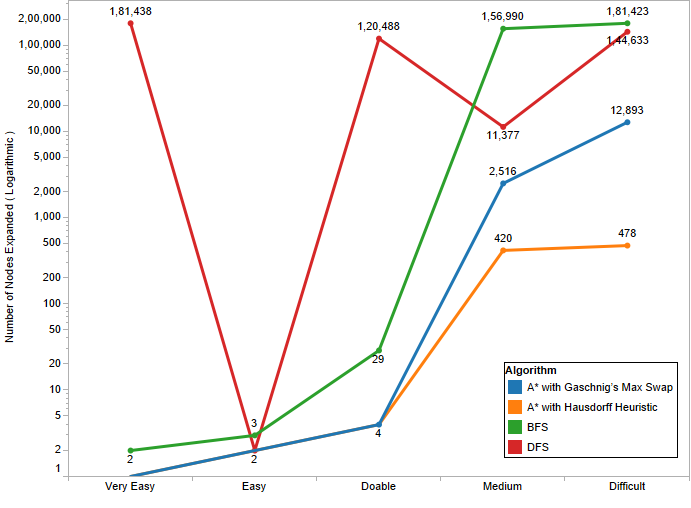
\includegraphics[width=\textwidth,keepaspectratio]{Images/Nodes_expanded.png}}
		\captionof{figure}{Nodes expanded}
		\label{fig:nodes}
	\end{minipage}
\end{table}

\noindent As shown in Figure~\ref{fig:nodes}, the number of nodes expanded for A* with both the heuristics is equal for very easy, easy and doable start states. However, for the medium and difficult start state, the number of nodes expanded has drastically decreased for A* with Hausdorff distance. For difficult start state, only 470 nodes are expanded for A* with Hausdorff distance as compared to 12,893 nodes for A* with Gaschnig's Max Swap. Also, the number of nodes expanded with all the start states (except easy) for A* with Hausdorff distance is less than the number of nodes for BFS and DFS. \\

\noindent It can be seen in Figure~\ref{fig:time} that the running time for A* with Hausdorff distance is greater than BFS and A* with Gaschnig's Max Swap for all the start states. However, as compared to DFS,  A* with Hausdorff distance takes lesser time for very easy and doable start states. \\

\noindent In terms of the cost of the path, we observed that BFS and A* with Gaschnig's Max Swap took an equal number of steps to reach the goal state. Figure~\ref{fig:cost} depicts the cost of the path where A* with Hausdorff distance took the same number of steps as BFS and A* with Gaschnig's Max Swap for very easy, easy and doable start states.  But it took more steps than these two algorithms for medium and difficult start states. In comparison to DFS, it performed better for doable, medium and difficult states. \\

\setlength{\intextsep}{5pt}
\begin{figure}
	\centering
	\begin{minipage}[b]{0.47\textwidth}
		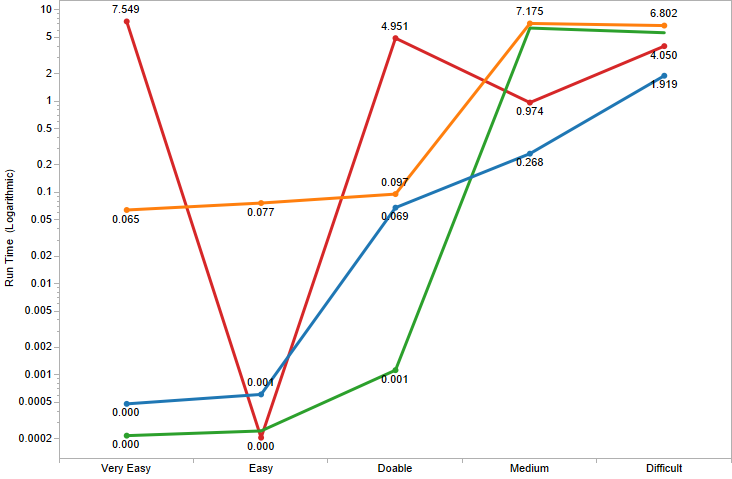
\includegraphics[width=\textwidth, height=4cm]{Images/RunningTime.png}
		\caption{Run Time}
		\label{fig:time}
	\end{minipage}
	\begin{minipage}[b]{0.47\textwidth}
		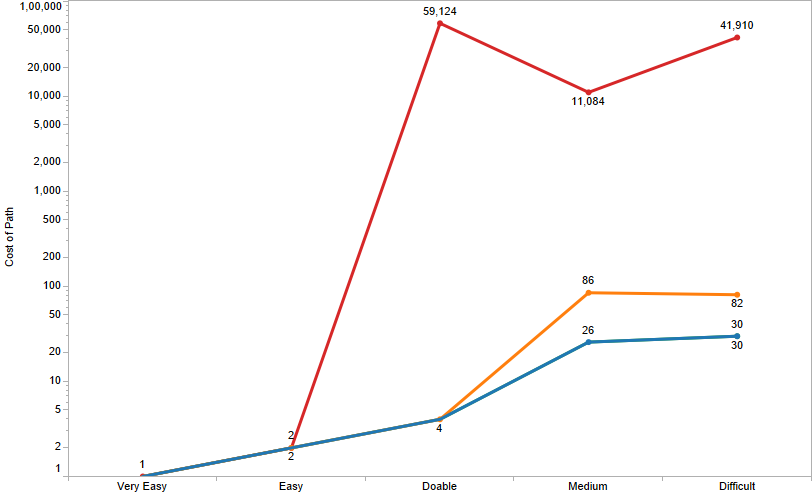
\includegraphics[width=\textwidth]{Images/costofpath.png}
		\caption{Cost of Path}
		\label{fig:cost}
	\end{minipage}\hfill
\end{figure}

\noindent  The analysis shows that A* with Hausdorff distance expands the least number of nodes as compared to all the baselines. However, it takes a larger running time because of the computations involved in image generation and image comparison. It was also observed that the cost of the path was more for this method as compared to BFS and A* with Gaschnig's Max Swap since it selects based on the newer heuristic value. Thus, this type of heuristic can be probably used in scenarios where image comparison is done such as solving jigsaw puzzles. \\

\section{Conclusions}
In this research, we applied BFS, DFS and A* algorithms to the 8-puzzle problem. We compared metrics such as the number of expanded nodes, cost of the path and running time of the algorithms. The A* algorithm outperforms the other two in most of these metrics. The comparison of heuristics on image puzzle has provided important insights about the practical application of Gaschnig's Max Swap and Hausdorff distance. Hausdorff distance evaluation function has shown promising results in our experiments and needs further research.

\begin{thebibliography}{6}
%

\bibitem {rus}
Russell,S., Norvig,P.: Artificial Intelligence: a Modern Approach:Prentice Hall, 2010.
\bibitem{tab}
Mathew,K., Tabassum,M., Ramakrishnan,M.: Experimental Comparison of Uninformed and Heuristic AI Algorithms for N Puzzle Solution (2013) 43-50. 
\bibitem{pea}
Pearl,J.,Korf,R.E.:Search Techniques: Annual Review Computer Science, Computer Science Department, University of California, Los Angeles, California  (1987) 451-467. 
\bibitem{shi}
Shih, H.,Lu, J.,Ma, C.: Solving Jigsaw Puzzles via Hausdorff-Based Border Compatibility: IEEE Conference on Multimedia Information Processing and Retrieval (MIPR), San Jose, CA, USA (2019) 504-505.
\bibitem{swa}
Swan, J.: Harmonic Analysis and Resynthesis of Sliding-Tile Puzzle Heuristics: IEEE, Department of Computer Science, University of York, Deramore Lane, York (2013) 516-524.

\end{thebibliography}
\end{document}
